\section{Main Technical Contributions}
\begin{frame}{CorrExt Construction Overview I}
%	\begin{itemize}
%		\item $ \IP[\bbK]^{[t]} \rightarrow \ROLE[\bbK] \rightarrow \OLE[\bbK]$, where $ \bbK = \GF{2^{\delta n}} $
%		\item Simultaneously embed $ \OLE[\GF 2]^m $ into one $ \OLE[\bbK] $
%		\item This embedding relies on finding solutions to a new combinatorial problem
%		
%		\TODO{draw a picture}
%	\end{itemize}
	\begin{definition}[Oblivious Linear-Function Evaluation (\OLE)]
		An oblivious linear-function evaluation over a field $ \bbF $
		\begin{itemize}
			\item represented as $ \OLE[\bbF] $
			\item takes $ (A,B) \in \bbF^2 $ from Alice, and $ X \in \bbF $ from Bob
			\item provides $ Z = AX +B $ to Bob 
		\end{itemize}  
	\end{definition}
	{\setbeamercolor{block title}{bg=Gray, fg=white}
	\begin{block}{Notes}
	\begin{itemize}
		\item Alice knows nothing about $ X $, and Bob knows nothing about $ A $.
		\item  \OT is functionally equivalent $ \OLE[\GF{2}] $ since $ x_b = (x_1 - x_0)b + x_0 $.
		%\item Random oblivious linear-function evaluation $ (\ROLE) $ is a randomized version of $ \OLE $.
	\end{itemize}
	\end{block}}
	
\end{frame}

\begin{frame}{CorrExt Construction Overview II}
	\begin{figure}
\onslide<1->{\small Goal: Alice and Bob want to produce $m$ {\OLE}s over \GF{2}.}
\hrule
\begin{center}

\begin{adjustbox}{max width={\textwidth}}
\begin{tikzpicture}[every node/.style={fill=white}, >=stealth]

%% Leaky IP
\onslide<2->{\node[draw, rectangle, align=center] (IP) {\IP[\bbK] with \\ $t$-bits\\leaked};}

%% OLE K
\onslide<3->{\node[draw, rectangle, right=.27\linewidth of IP, align=center] (OLEk) {\underline{one}\\\OLE[\bbK]};}

%% m-OLE
\onslide<4->{\node[draw, rectangle, right=.27\linewidth of OLEk, align=center] (mOLE) {$m$ copies of\\ \OLE[\GF{2}]};}

\begin{pgfonlayer}{background}

%% second arrow
\onslide<4->{\draw[thick, ->] (OLEk) -- (mOLE) node[above, midway, fill opacity=0, text opacity=1] {\footnotesize \OLE[]-Extraction};}

\onslide<5>{
%% first cloud
\node[draw, cloud, cloud ignores aspect, fit=(IP.center)(OLEk.center), cloud puffs=15, inner ysep=1.7em, inner xsep=1.2em] (cloud1) {};
}

%% first arrow
\onslide<3->{\draw[thick, ->] (IP) -- (OLEk) node[above, midway, align=center,fill opacity=0, text opacity=1] {\footnotesize Random-Output\\\footnotesize Correlation Extractor};}

\onslide<6->{
%% second cloud
\node[draw, cloud, cloud ignores aspect, fit=(OLEk.center)(mOLE.center), cloud puffs=17, inner ysep=1.5em, inner xsep=1em] (cloud2) {};

%% second arrow (again)
\draw[thick, ->] (OLEk) -- (mOLE) node[above, midway,fill opacity=0, text opacity=1] {\small \OLE[]-Extraction};
}


\end{pgfonlayer}


\end{tikzpicture}
\end{adjustbox}

\end{center}
\end{figure}
	\only<2>{Natural generalization of \cite{C:GIMS15} protocol for \IP[] to arbitrary fields.}
	\only<3,4>{Embed $ m $ copies of $\OLE[\GF{2}] $ into \underline{one} $ \OLE[\bbK] $}
	\only<4>{\setbeamercolor{block title}{bg=Gray, fg=white}
		\begin{block}{Notes}
			\begin{itemize}
				\item This embedding relies on finding solutions to a combinatorial problem.
				\item The bigger value of $ m $, the better production rate.
			\end{itemize}
		\end{block}
	}
\end{frame}

\begin{frame}{Our Combinatorial Problem}
	
	{\setbeamercolor{block title}{bg=ForestGreen, fg=white}
	\begin{block}{Our Combinatorial Problem}
		Find two ordered sets $ S = (s_1, s_2, \cdots, s_m) $ and $ T = (t_1, t_2, \cdots, t_m) $ \st
		\begin{itemize}
			\item $ s_i, t_i $ are non-negative integers
			\item $ s_i + t_i < n $
			\item $ s_i + t_i \neq s_j + t_k  $ for every $ i, j, k $ that are not simultaneously equal
			\item $ m $ is maximized 
		\end{itemize} 
	\end{block}}
	\pause

	{\setbeamercolor{block title}{bg=Gray, fg=white}
	\begin{block}{Notes}
		\begin{itemize}
			\item This problem is a generalization of the 3-free set (sets that avoid any arithmetic progressions of length 3) problem.
			\item Using the 3-free set, we get $ m = n^{1-o(1)} $.
		\end{itemize}
		
	\end{block}}

	\pause
	\begin{lemma}
		Recently we show that $ m = o(n) $.
	\end{lemma}
\end{frame}

\begin{frame}{Our Embedding Problem}
	\begin{itemize}
	\item Our aim: Suppose there is an oracle that performs OLE over an extension field $ \bbK $. By making only one call to this oracle, no other communication allows, how many OLEs over the field $ \bbF $ can be calculated? %\pause
	\item More concretely: 
	\begin{itemize}
		\item Given an oracle that take as input $ A, B \in \bbK  $ from Alice and $ X \in \bbK $ from Bob, and outputs $ Z = A\cdot X + B $ to Bob. %\pause
		
		\item  Alice: $ (a_0, a_1, \cdots, a_{m-1}) \in \bbF^m $ and $ (b_0, b_1, \cdots, b_{m-1}) \in \bbF^m $. %\pause
		\item  Bob: $ (x_0, x_1, \cdots, x_{m-1}) \in \bbF^m $. %\pause
		\item  We want Bob to obtain $ (z_0, z_1, \cdots, z_{m-1}) \in \bbF^m $, where $ z_i = a_i \cdot x_i + b_i $. %\pause
		\item Intuitively, we want to maximize $ m $ and embed $ OLE(\bbF)^m $ into one $ OLE(\bbK) $ %\pause
	\end{itemize}
	\item Easy to embed for $ m = 1 $ but can we do better? 
\end{itemize}
\end{frame}

\begin{frame}{Embedding}
	\begin{itemize}
		\item Given $ S = (s_0, s_1, \cdots, s_{m-1}) $ and $ T = (t_0, t_1, \cdots, t_{m-1}) $ to be a solution to the combinatorial problem. %\pause
		\item $  A = \sum_{i = 0}^{m-1} a_i \zeta^{s_i} $ %\pause
		\item $ B = \sum_{i=0}^{n-1} r_i \zeta^i $, where \\ $ r_i = \begin{cases}
		b_k & ,\text{ if } i = s_k + t_k \text{ for some } k \in \{0, 1, \cdots, m-1\} \\
		U_{\bbF} & ,\text{ otherwise.}
		\end{cases} $ %\pause
		\item $ X = \sum_{i=0}^{m-1} x_i \zeta^{t_i} $ %\pause
		\item Invoke the oracle, Bob receives $ Z = AX + B $. %\pause
		\item $ A X = \sum\limits_{i,j} a_i x_j \zeta^{s_i + t_j} = \sum\limits_{i} a_i x_i \zeta^{s_i + t_i} + \sum\limits_{j \neq k} a_j x_k \zeta^{s_j + t_k} $. %\pause
		\item The coefficient of $ \zeta^{s_i + t_i} $ in $ Z $ is $ z_i = a_i x_i + b_i $ since $ s_i + t_i \neq s_j + t_k $.
	\end{itemize}
	
\end{frame}

\begin{frame}{Simple Partition Number}
	\begin{definition}
		A \textit{simple graph} is a bipartite graph such that each of its
		connected component is a biclique
	\end{definition}
	\pause
	\begin{definition}
		The \textit{simple partition number} of a bipartite graph $G$, represented
		by $\sp G$, is the minimum number of simple graphs needed to
		partition its edges.
	\end{definition}
	\pause
	\begin{figure}[htb] \footnotesize
\begin{center}
\begin{tikzpicture}[
  vert/.style = {node distance = 5mm, circle, draw, fill = purdue-gold!40, thick, inner sep = 1pt},  
  bdd/.style = {rectangle, draw, inner sep = 5mm}, 
                   ]

%%% First Correlation 
\node [vert] (a00) at (0,0) {00}; 
\node [vert, below = of a00] (a01) {01}; 
\node [vert, below = of a01] (a10) {10}; 
\node [vert, below = of a10] (a11) {11}; 

\node [vert, node distance = 10mm, right = of a00] (b00) {00}; 
\node [vert, below = of b00] (b01) {01}; 
\node [vert, below = of b01] (b10) {10}; 
\node [vert, below = of b10] (b11) {11}; 


\draw [thick] (a00) -- (b00)  (a00) -- (b01)  (a00) -- (b10)  (a00) -- (b11); 
\draw [thick] (a01) -- (b00)  (a01) -- (b10); 
\draw [thick] (a10) -- (b00)  (a10) -- (b01); 
\draw [thick] (a11) -- (b00)  (a11) -- (b11); 

%\pause 

\node at (2.3,-1.7) {=}; 

\node [vert] (c00) at (3,0) {00}; 
\node [vert, below = of c00] (c01) {01}; 
\node [vert, below = of c01] (c10) {10}; 
\node [vert, below = of c10] (c11) {11}; 

\node [vert, node distance = 10mm, right = of c00] (d00) {00}; 
\node [vert, below = of d00] (d01) {01}; 
\node [vert, below = of d01] (d10) {10}; 
\node [vert, below = of d10] (d11) {11};

\draw[draw=red!70!black, thick] (c00) -- (d00)  (c00) -- (d11);
\draw[draw=blue!70!black, thick] (c01) -- (d10);
\draw[draw=green!70!black, thick] (c10) -- (d01);
\draw[draw=red!70!black, thick] (c11) -- (d00)  (c11) -- (d11);


\node at (5.3, -1.7) {+};

\node [vert] (e00) at (6,0) {00}; 
\node [vert, below = of e00] (e01) {01}; 
\node [vert, below = of e01] (e10) {10}; 
\node [vert, below = of e10] (e11) {11}; 

\node [vert, node distance = 10mm, right = of e00] (f00) {00}; 
\node [vert, below = of f00] (f01) {01}; 
\node [vert, below = of f01] (f10) {10}; 
\node [vert, below = of f10] (f11) {11};

\draw[draw=red!70!black, thick] (e00) -- (f01)  (e00) -- (f10);
\draw[draw=green!70!black, thick] (e01) -- (f00);
\draw[draw=green!70!black, thick] (e10) -- (f00);


\end{tikzpicture}
\end{center}
%\caption{A decomposition of $ \IP {} $ into 2 simple graphs.}
\label{fig:IP^2-sp-decomp}
\end{figure}





\end{frame}

\begin{frame}{Connection between Maximum Leakage and Simple Partition Number}
	\begin{lemma}[Connecting Max. Resilience to $\sp G $]
		Suppose $ G = (R_A, R_B) $ is a correlation and there exist $\Lambda$ simple graphs $ G^{(1)}, G^{(2)}, \cdots, G^{(\Lambda)} $ that partition the edges of the graph $ G $. 
		Then $ G $ is not resilient to $ \log \Lambda $ bits of leakage.
	\end{lemma}
	\pause
	
	\begin{block}{Intuition}
		Small simple partition number implies low maximum leakage resilience
	\end{block}
	\pause
	\underline{Proof outline.} 
	\begin{itemize}
		%\item Consider $ \pi $ resilient to $ \log \Lambda $-bit leakage and securely implements one $\pred{OLE} $.
		\item Consider the leakage $ \cL: E(G) \rightarrow [\Lambda] $ \st $ \forall e \in E(G), \cL(e) = \ell $ and $ e \in E(G^{(\ell)}) $ 
		\item Conditioned on the leakage being $ \ell $, the correlaiton $ (R_A, R_B | \ell) \equiv G\p\ell$ is a simple correlation 
		\item Simple correlations are useless for correlation extractor by \cite{}.
	\end{itemize}

\end{frame}

\begin{frame}{Estimating Simple Partition Number}
	\begin{figure}
\begin{center}
%\begin{table}
{\renewcommand{\arraystretch}{2}
\begin{tabular}{|c|c|c|c|}\hline
Correlation & Secret Share & Simple Partition  & Fractional Leakage\\
Description & Size (s) & Number (\pred{sp}) & Bound ($\log\pred{sp}/s$)\\\hline 
$\ROT[n/2]$ & $n$ & $2^{n/4}$ & \begin{adjustbox}{valign=m}
\begin{tikzpicture}
	\only<1,3->{\node[] {1/4};}
	\only<2>{\node[draw, red, circle, ultra thick, inner sep=2pt] {\textcolor{black}{1/4}};}
\end{tikzpicture}
\end{adjustbox} \\\hline 
%$\ROLE[\bbF]^{n/2}$ & $n\log\abs\bbF$ & $\abs{\bbF}^{n/4}$ & $1/4$\\\hline
$\IP[\bbF^n]$ & $n\log\abs\bbF$ & $\abs{\bbF}^{n/2}$ & $1/2$\\\hline 
\end{tabular}
%\begin{tabular}{| c | c | c | c | c | c |}\hline 
%& Correlation & Number of \OT{}s  & Number of & Simulation  & Round\\
%& Description  & Produced $(m)$ & Leakage bits $(t)$ & Error $(\eps)$ & Complexity \\\hline
%\cite{FOCS:IKOS09} & \ROT[n/2] & $\alpha n$ & $\beta n$ & $2^{-\gamma n}$ & 4\\\hline
%\multirow{2}{*}{\cite{C:GIMS15}} & \ROT[n/2] & $n/\poly\log n$ & $(\nicefrac14 - g) n$ & $2^{-g n/m}$ & 2 \\\cline{2-6} 
%& \IP[\GF{2}^{n}] & $1$ & $(\nicefrac12 - g) n$ & $2^{-gn}$ & 2\\
%\hline\hline
%%Our Work & \ROLE[\GF{2^n}] & $n^{1-o(1)}$ & $(\nicefrac12 - g) n$ & $2^{-gn}$ & 2\\\hline 
%Our Work & \IP[\bbF^{n/\log\abs\bbF}] & $n^{1-o(1)}$ & $(\nicefrac12 - g) n$ & $2^{-gn}$ & 2\\\hline 
%\end{tabular}
%\end{tabular}
}
\end{center}
%\caption{
%  A summary of the estimates of the simple partition number for the correlations relevant to our work.   
%}
\label{fig:sp} 
\end{figure}







	{\setbeamercolor{block title}{bg=Gray, fg=white}
		\begin{block}{Note}
			\begin{itemize}
				\item $ s $ is the secret share size
				\item $ (\log \pred{sp})/s $ is the upper bound on the maximum leakage resilience.
			\end{itemize}
		\end{block}
	}
%	\begin{lemma}
%		$ \sp{\IP ({\bbF^n})} \leq \abs{\bbF} ^{\ceil{(n+1)/2}}$
%	\end{lemma}
\end{frame}

\begin{frame}{Relevant Prior Work on Common Information}

	{\setbeamercolor{block title}{bg=red, fg=white}
	\begin{block}{Mutual information $ I(R_A, R_B) $}
		\begin{itemize}
			\item $ \# $ bits of the secret key that two parties can agree on
		\end{itemize}
	\end{block}}
	\pause
	{\setbeamercolor{block title}{bg=brown, fg=white}
	\begin{block}{\gacs-\korner \cite{} common information  $ K(R_A, R_B) $}
		\begin{itemize}
			\item The largest entropy of the common random variable that each party can generate based on their respective secret share
			\item Corresponding to \textit{number of connected components}
		\end{itemize}
	\end{block}}
	\pause
	{\setbeamercolor{block title}{bg=blue, fg=white}
	\begin{block}{Wyner's common information \cite{} $ J(R_A, R_B) $}
		\begin{itemize}
			\item Min. amount of leakage that kills the possibility of key agreement
			\item Corresponding to \textit{biclique partition number}
		\end{itemize}
	\end{block}}
\end{frame}

